\documentclass{beamer}
\usepackage{graphicx}

\usetheme{Madrid}
\usecolortheme{beaver}
\setbeamertemplate{navigation symbols}{}

\title{Mathematics in Deep Learning}
\author{Lachlan Jones}
\institute{Math199}
\date{2024}

\begin{document}

\frame{\titlepage}

\begin{frame}
    \frametitle{A classification problem}
    Let's build some networks to seperate this dataset of red and blue dots
    \begin{figure}
        \centering
        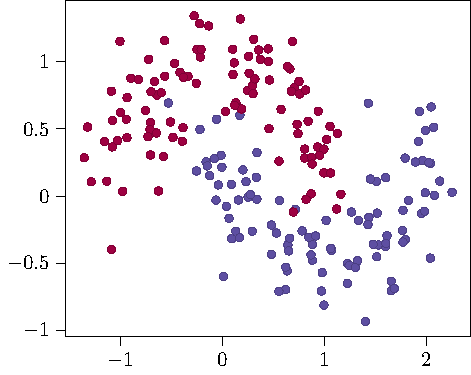
\includegraphics{./figures/moons/main.pdf}
    \end{figure}
\end{frame}

\begin{frame}
    \frametitle{Simple perceptron networks}
    Perceptrons are the building block of Neural Networks
    \begin{figure}
        \centering
        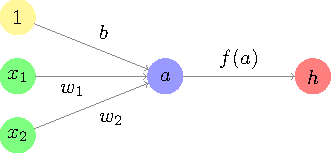
\includegraphics{./figures/simple-perceptron/main.pdf}
        \caption{Simple perceptron network with two inputs}
    \end{figure} \pause
    \begin{itemize}
        \item \(a = w_1 \cdot x_1 + w_2 \cdot x_2 + b\) \pause
        \item \(f\) is a \alert{non-linear activation function} \pause
        \item the weights \(w_1\) and \(w_2\) and bias \(b\) are \alert{parameters}
    \end{itemize}
\end{frame}

\begin{frame}
    \frametitle{Simple perceptron networks}
    Limited to linear decision boundaries:
    \begin{figure}
        \centering
        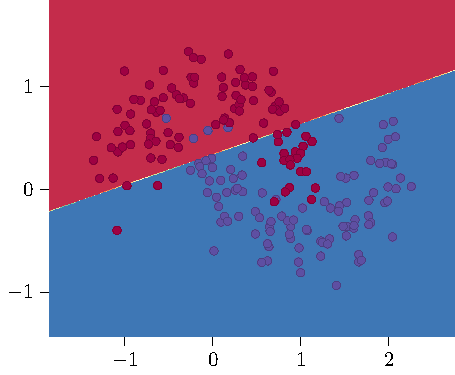
\includegraphics[height=0.6\textheight]{figures/linear-boundary/main.pdf}
        \caption{Simple perceptron decision boundary}
    \end{figure}
\end{frame}

\begin{frame}
    \frametitle{MLP networks}
    \begin{itemize}
        \item Multi-layered perceptron
        \item Combine multiple perceptrons together into a large network
    \end{itemize}
\end{frame}

\begin{frame}
    \frametitle{MLP networks}
    \begin{figure}
        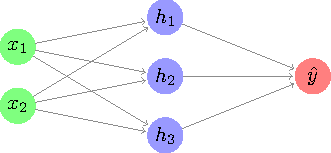
\includegraphics{figures/basic-mlp/main.pdf}
        \caption{MLP network with two inputs and one hidden layer}
    \end{figure}
    \begin{block}{Remark}
        We've tidied up our diagram to not have biases and activation functions, but they're still used in calculations.
    \end{block}
\end{frame}

\begin{frame}
    \frametitle{MLP networks}
    Calculations:
    \[a_{1} = w_{1, 1} \cdot x_1 + w_{1, 2} \cdot x_2 + b_{1}\]
    \[a_{2} = w_{2, 1} \cdot x_1 + w_{2, 2} \cdot x_2 + b_{2}\]
    \[a_{3} = w_{3, 1} \cdot x_1 + w_{3, 2} \cdot x_2 + b_{3}\] \pause
    This is a typical system of equations, so we can tidy things up with matrix algebra: \pause
    \[
        \begin{bmatrix}
            a_{1} \\
            a_{2} \\
            a_{3}
        \end{bmatrix}
        =
        \begin{bmatrix}
            w_{1, 1} & w_{1, 2} \\
            w_{2, 1} & w_{2, 2} \\
            w_{3, 1} & w_{3, 2} \\
        \end{bmatrix}
        \begin{bmatrix}
            x_1 \\
            x_2
        \end{bmatrix}
        +
        \begin{bmatrix}
            b_1 \\
            b_2 \\
            b_3
        \end{bmatrix}
    \] \pause
    With an activation function, the output of the hidden layer is:
    \[\underline{h} = f(W \cdot \underline{x} + \underline{b})\]
\end{frame}

% \begin{frame}
%     \frametitle{MLP networks}
%     Typically, architecture is much more complex:
%     \begin{figure}
%         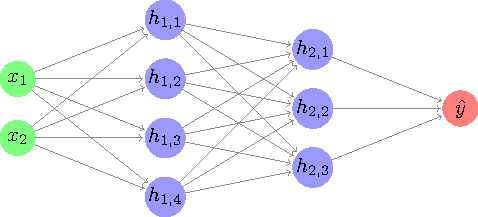
\includegraphics{figures/mlp/main.pdf}
%         \caption{MLP network with two inputs and two hidden layers of different sizes}
%     \end{figure}
% \end{frame}

\begin{frame}
    \frametitle{MLP networks}
    Typically, we have many hidden layers in our network architecture.
    \vspace{0.5cm}

    Generally:
    \[\underline{h}_i = f(W_i \cdot \underline{h}_{i - 1} + \underline{b}_i)\] \pause
    \begin{block}{Remark}
        We can think of the network as a recurrence relation, passing the output of one hidden layer as the input to the next layer.
    \end{block}
\end{frame}

\begin{frame}
    \frametitle{MLP networks}
    The combination of \alert{hidden layers} and \alert{non-linear activation functions} gives us a \alert{non-linear decision boundary}:
    \begin{figure}
        \centering
        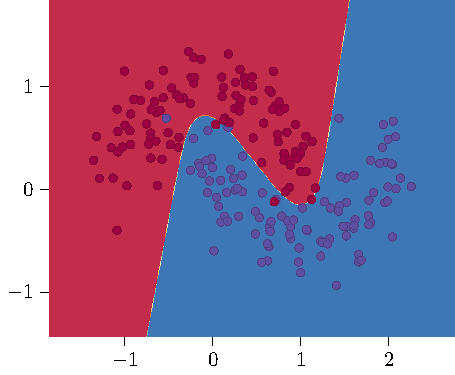
\includegraphics[height=0.6\textheight]{figures/non-linear-boundary/main.pdf}
        \caption{MLP decision boundary}
    \end{figure}
\end{frame}

\begin{frame}
    \frametitle{Training}
    \begin{itemize}
        \item Networks don't just magically start with great performance, we have to \alert{train} them on our dataset. \pause
        \item \alert{Training} is achieved by updating our \alert{parameters}, the weights and biases. \pause
        \item We achieve this using \alert{calculus}.
    \end{itemize}
\end{frame}

\begin{frame}
    \frametitle{Training}
    We define a \alert{loss function} that depends on the parameters:
    \[J(\theta_1,... , \theta_n)\]
    A loss function compares the error of a network's current prediction against human labelling of data. 
    \vspace{0.5cm}

    We want to find a local minima of this function. 
\end{frame}

\begin{frame}
    \frametitle{Training}
    We can compute the \alert{gradient} of the loss function, which tells us how to make small updates to our parameters:
    \[\nabla J(\theta_1,... , \theta_n) = \begin{bmatrix}
        \frac{\partial J}{\partial \theta_1} \\[6pt]
        \frac{\partial J}{\partial \theta_2} \\[6pt]
        \vdots \\[6pt]
        \frac{\partial J}{\partial \theta_n}
    \end{bmatrix}\]
    These are partial derivatives with respect to each parameter. You'll learn about partial derivatives later in semester 2. 
\end{frame}

\begin{frame}
    \frametitle{Training}
    A great way to visualise this is walking down a mountain, the gradient tells us the steepest way down. 
    \begin{figure}
        \centering
        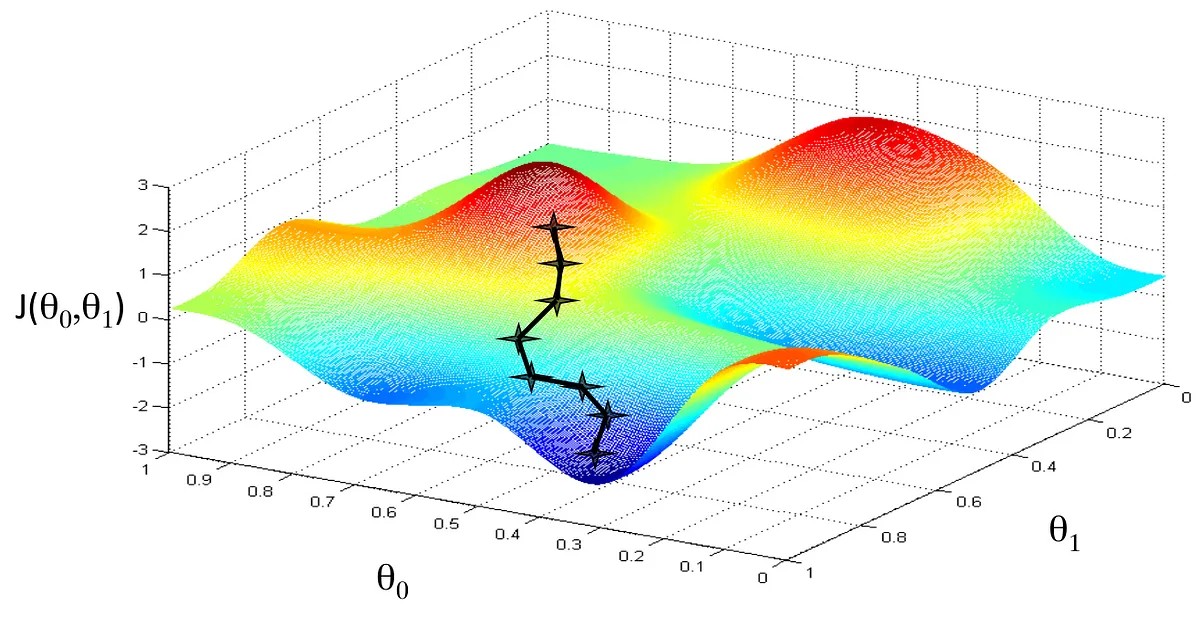
\includegraphics[width=0.8\textwidth]{images/gradient-descent.png}
    \end{figure}
\end{frame}

\begin{frame}
    \frametitle{Conclusion}
    These are the foundational concepts that are used in advanced architecture:
    \begin{figure}
        \centering
        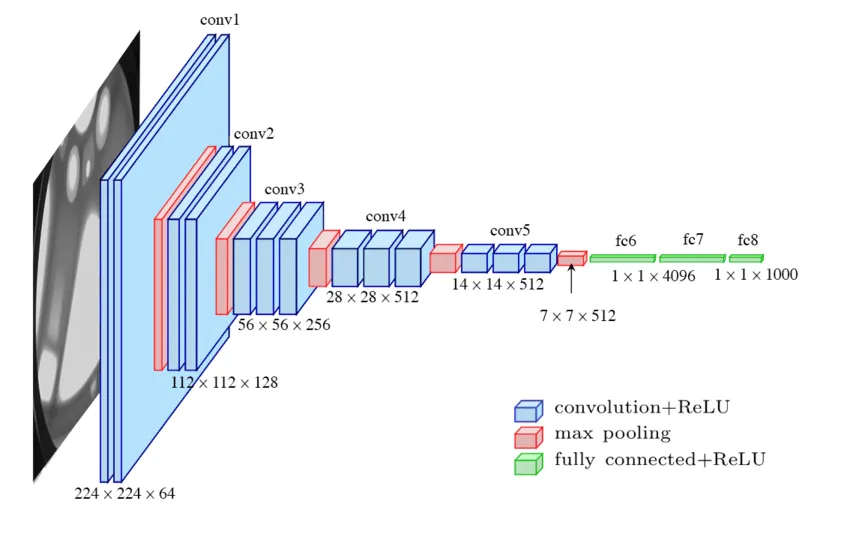
\includegraphics[width=0.7\textwidth]{images/vgg-architecture.png}
    \end{figure}
    While they may seem scary, neural networks are just algebra and calculus.
\end{frame}

\begin{frame}
    \frametitle{Will AI take over?}
    At the end of the day, neural networks are simply matching a trend to some data:
    \begin{figure}
        \centering
        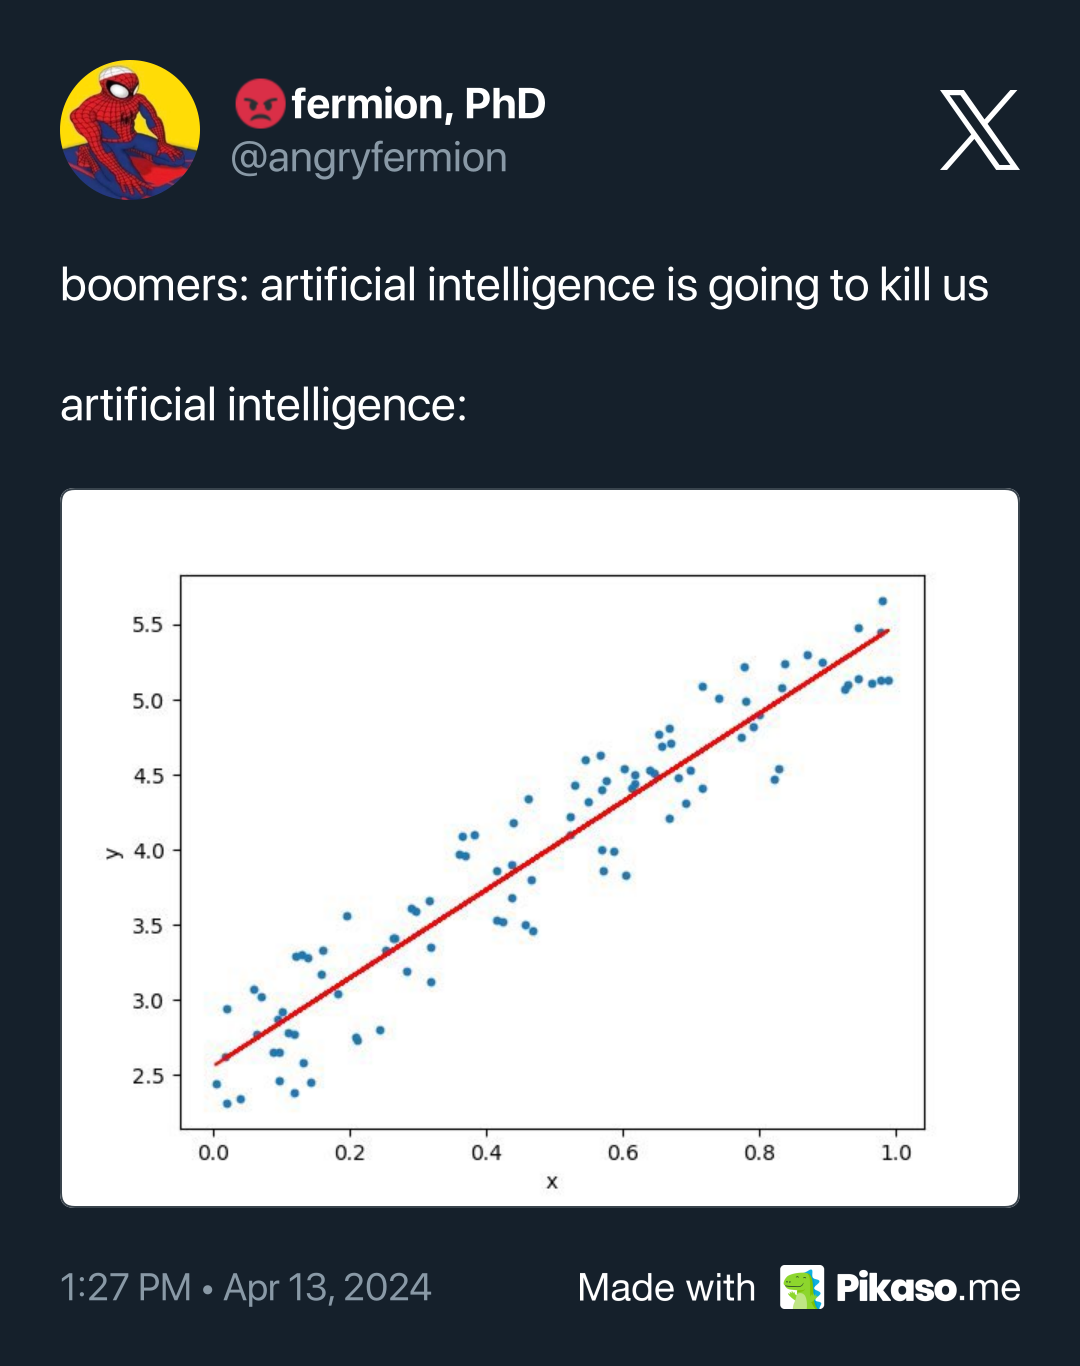
\includegraphics[height=0.75\textheight]{./images/pikaso.me-angryfermion-20240413_132756-1779139460174676132.png}
    \end{figure}
\end{frame}

\end{document}